% !TeX spellcheck = <none>
\documentclass[11pt,a4paper]{article}
% Change Hons to PhD, MAE, MPhil or MComm as appropraite
% Remove singlespace and singleside for final version.

\usepackage{float,fullpage}
\usepackage{gensymb}
\usepackage{natbib}
\usepackage{pdfpages}
\usepackage{listings}

\title{Predicting Fire Risk: \\ An Evaluation of the Fire Danger Index}
\author{Elle Saber, Rob J Hyndman \& Di Cook}


\begin{document}
\maketitle

\section*{Abstract}

This paper investigates the effectiveness of the Forest Fire Danger Index (FFDI) \citep{mcarthur67} at predicting probability of ignition of bushfire in Victoria using logistic regression, classification trees and random forests. I construct a 10km gridded dataset of Victoria consisting of daily values for FFDI, temperature, wind speed, relative humidity, the drought factor, grassland curing level, vapour pressure at 9am and precipitation between 2000 and 2010. I find that the FFDI alone is a poor predictor of ignition. By adding the input variables to the FFDI, grassland curing, vapour pressure at 9am and precipitation I improve model accuracy and conclude that, of the variables used, grassland curing is the most important in predicting ignition. Combining non-linear regression splines with logistic models produces predictive performance comparable with random forests. 

\section{Introduction}

In Australia, bushfires are one of the most common natural disasters impacting lives and property. To minimise the damage from fire occurence, management agencies often allocate resources according to where fires are expected to occur and where fire behaviour could be more severe  \citep{padilla11, wotton05}. In order to plan effectively and manage risks resulting from bushfire, the measures used to predict fire occurrence and severity must be reliable and accurate.  

There is limited literature on the effectiveness of the Australian fire danger rating system using statistical techniques, the majority of Australian research uses case studies. Internationally research on fire danger rating systems use standard econometric techniques such as logistic regression or heckman sample selection models. Machine learning and non-parametric estimation are not used extensively in this area. 

This paper uses the Australian Forest Fire Danger index (FFDI) as a baseline model for predicting probability of ignition of bushfire then investigates strategies to improve the accuracy of the predictor. Given the science of combustion and fire behaviour it is highly unlikely that the factors affecting fire ignition impact the probability in a linear manner or without interacting with each other. 

I construct a dataset of bushfire ignition and metereological variables such that predicting fire ignition becomes a binary classification problem. Then I apply both some common machine learning techniques: classification trees and random forests and compare their performance to logistic regression models which use non-parametric smoothing functions. The dataset suffers from severe class imbalance, the number of fires compared to number of non fires is tiny. Accordingly, models are evaluated based on balance accuracy measures and reciever operating characteristic plots. 

 The greatest improvement in accuracy occurs in models which allow for the input variables to behave non-linearly. By adding spline functions to the logistic model I produce a predictor which is comparable to the random forest in accuracy. 

While the FFDI may be a good measure of fire intensity once ignition occurs, it is a poor predictor of fire ignition. Predictor performance is improved with the inclusion of the FFDI input variables, grassland curing, vapour pressure at 9am and precipitation. Specfically of these variables, grassland curing is the most important variable in determining probability of ignition. 


\section{Background and Literature Review}

\subsection{Fire Danger Rating Systems and McArthur's Forest Fire Danger Index}
Fire danger rating systems estimate the severity of burning conditions and likelihood of fire over a large area at a particular time \citep{chandler83, andrews03}. The Forest Fire Danger Index (FFDI) \citep{mcarthur67} is the fire danger rating system used in Australia. It integrates weather elements into an index and is used as a key tool in assessing fire danger in Australia. Fire danger rating indices are accepted worldwide for anticipating general fire activity in a given area but less so for evaluating ignition probabilities. 

McArthur’s FFDI originated as tabulated indices and were subsequently reduced to equations by \citet{noble80} which in turn simplified into the formulation of the FFDI given by equation (\ref{eq FFDI}). 

\begin{equation}
\label{eq FFDI}
F=2.0 e^{-0.450 + 0.987 \ln(D)-0.0345H+0.0338T+0.0234V}
\end{equation}
where 
\begin{itemize}
	\item $D$: drought factor (Index)
	\item $H$: relative humidity (percent)
	\item $T$: temperature (degrees Celsius)
	\item $V$: Average wind velocity (\emph{km/hr})
\end{itemize}

McArthur's FFDI relates weather conditions to expected fire behaviour and rate of spread. It is used in fire fighting operations by weather forecasters and fire agencies to determine fire danger \citep{clarke2013}. 

\begin{table}[ht]
	\centering
	\begin{tabular}{|c|c|}
		\hline Fire Danger Rating & Forest Fire Danger Index \\ 
		\hline
		Low-Moderate  & 0-11 \\ 
		High  &  12-24 \\ 
		Very High  &  25-49\\ 
		Severe &  50-74\\ 
		Extreme  &  75-99 \\ 
		Code Red  &  100+ \\ 
		\hline 
	\end{tabular}
	\caption{The Forest Fire Danger Index and the Fire Danger Rating}
	\label{table:FDR}
\end{table}

While the FFDI has been the most universally accepted fire danger rating system used in Australia for many decades, there are a number of weaknesses which may compromise its ability to accurately predict severe fire. 

\begin{enumerate}
	\item Experimental studies conducted during its development largely focused on small scale fires in very specific types of forests and under only moderate weather conditions. 
	\item The most severe conditions represented by the FFDI were based on known worst case scenario fires, specifically the 1939 Black Friday fires.
\end{enumerate}

These factors limit the applicability of the FFDI in situations where the weather conditions may be out of these envisioned ranges. This is precisely the situation which occurred on Black Saturday 2009 \citep{harris12}. 

There is extensive research on predicting fire behaviour using meteorological and topographical information given ignition occurence but comparatively little also on  predicting fire occurrence and on evaluating the McArthur index. 

\citet{dowdy10} produced an extensive report on Australian fire weather, sensitivity analyses and the relationship between the FFDI and Canadian Fire Weather Index concluding that both indices were most sensitive to temperature and windspeed. Importantly \citet{dowdy10} found in some areas of Australia (Eastern Victoria, Tasmania and south west Western Australia) significant fire activity corresponds with relatively low index values suggesting that the value of the FFDI alone may not be a good predictor of fire activity. 

Evaluations of other fire danger indices and weather related indices around the world have used statistical techniques as simple as correlation, and as sophisticated as logistic regression (\cite{andrews03}; \cite{harris14}). 

%The only work comparing the FFDI to the FWI is a case study involving a pine plantation fire, the FWI was evaluated in direct comparison to the FFDI  and was found to be the better predictor of extreme fire behaviour \citep{cruz07}. This study will fill this gap in the literature by using statistical analysis to evaluate the performance of the FFDI. 

\subsection{Predicting fire activity}
A study linking fire activity to certain climate variables (some of which are inputs to the FFDI, others of which are not) and the El Niño Southern Oscillation (ENSO) index found significant relationships between fire activity and vapour pressure, maximum and minimum temperature and antecedent rainfall \citep{harris14}. Notably the variables which the indices are most sensitive to are different to those found to have the strongest link with fire activity suggesting that the fire danger indices may not contain all the important information for predicting fire activity \citep{harris14}. 

Logistic regression is common in studies predicting fire activity. The Bushfire and Natural Hazards Cooperative Research Center used logistic regression over daily historical rasters to predict probability of ignition (Read et al., 2015). Similarly, studies in Europe have used logistic regression with socio-economic factors or geographic features as dependent variables rather than fire danger ratings \citep{del11, zhang13}. 

There is some literature from Europe and the U.S. on evaluating Fire Danger Rating systems, specifically the U.S. Fire Danger Rating System and the Canadian Fire Weather Index.  These investigations of fire danger rating systems and fire occurrence have  generally used logistic regression \citep{andrews03, padilla11}. 

\section{Data}

The CFA divides the state into different districts for management purposes. I use these districts to capture different terrain types, fuel types and population density in Victoria. Dividing the data into these districts allows us to observe any difference in the behaviour of the variables across different parts of the state. Figure \ref{fig:dist} shows a map of the districts and their labels. 

\begin{figure}[h]
	\centering 
%	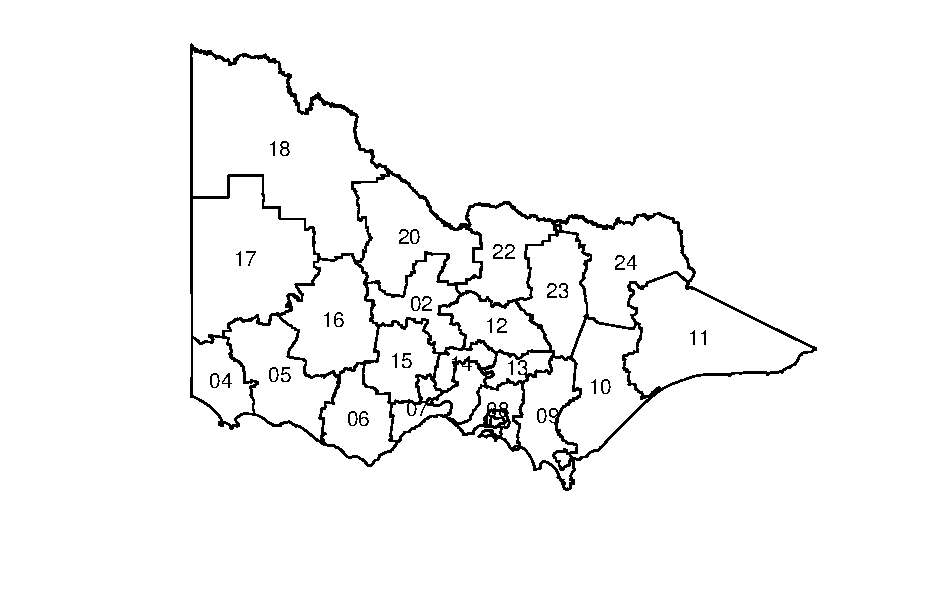
\includegraphics[width=1\columnwidth]{figures/Data/cfadis.pdf} 
	\caption{Country Fire Authority Districts} 
	\label{fig:dist} 
\end{figure}

\subsection{Explanatory Variables}

In this thesis, I predict probability of ignition using McArthur's Forest Fire Danger Index (FFDI), the meteorological variables used as inputs for the FFDI, grassland curing, vapour pressure at 9am and rainfall.  

\subsubsection{Weather}

The metereological data set comes from a climate simulation of the Murrary Darling Basin using the Weather Research and Forecasting (WFR) model. The WRF Modeling system has been developed by the National Center for Atmospheric Research (NCAR), the National Oceanic and Atmospheric Administrations Centers for Environmental Predicion (NCEP) and the other weather research institutions in the United States. \citet{evans10} used the Advanced Research WFR version 3 \citep{skamarock08} to simulate weather for southeastern Australia at a 10km horizontal grid over 24 years from 1985.

One weakness of this dataset is the fact it is modeled rather than observed. While actual observations would be ideal, there is no observational data at this resolution for this length of time in Australia. \citet{lucas10} developed a historical fire weather data set for 78 Bureau of Meteorology weather stations located around Australia. Not long after, an assessment of quality of this data set by \citet{clarke2013} revealed that only 38 of Lucas's 78 stations could be considered good quality. 38 geographical points over the whole country is too sparse a dataset to be feasible for this project. 

The strengths of the dataset make up for its shortcomings. As discussed, the resolution of the WRF model gives a grid resolution not possible from observations. \citet{evans10} evaluate the model output against gridded precipitation and temperature observations available from the Australian Water Availability Project and it was deemed to have successfully reproduced daily statistics capturing spatial patterns  \citep{evans10, clarkeevans13}. An additional advantage of using modelled data is that there are no missing values or false readings from weather stations to create problems in analysis. 

The FFDI data is created with the metereological variables from the WRF model. As per \citet{clarkeevans13} the spatial distribution of the FFDI has also been evaluated against observations with success  \citep{sanabria13}. Clarke and Evans discuss some heterogenieties with modelled windspeed due to changing technology used to measure this variable mostly evident in rural areas before the 1990s resulting in an underestimation of average FFDI values by approximately 5 percent for this period. The fire occurence dataset begins in 2000 and as a result these windspeed errors do not impact my analysis.

The WRF model \citep{evans10} is deemed to be an accurate representation of Australian weather on this scale and is a useful tool for modelling fire weather over Australia \citep{clarke2013}. The paper uses the FFDI, maximum temperature (Kelvin), wind speed (m/s), relative humidity (\%) and the drought factor calculated by \citet{clarke2013}  from this model. All other variables used in this paper are matched to the 10km gridpoints in the meteorological dataset. 

%Graphs, need to redo better
\begin{figure}[h]
	\centering 
%	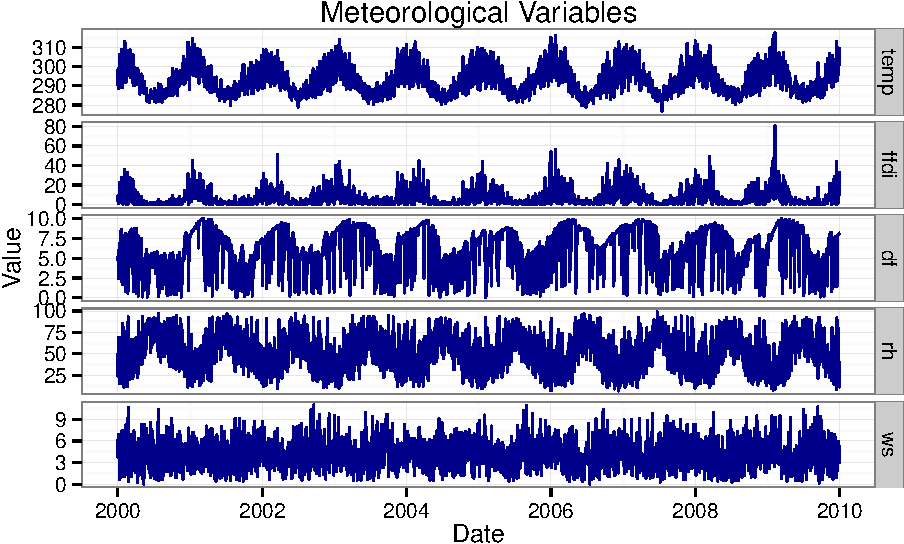
\includegraphics[width=1\columnwidth]{figures/Data/silvan.pdf} 
	\caption{Time series of meterological varibles for Silvan (-37.82, 145.42)} 
	\label{fig:silv} 
\end{figure}

Figure \ref{fig:silv} shows the time series of the meteorological variables for one point in Victoria. The temperature variable is the daily maximum, values are given in Kelvin (\degree C = K - 273.15), and we clearly observe the seasonal cycles with higher temperatures in the summer months and lower temperatures in the winter months. Maximum daily temperatures across the state range from around 2 \degree C to 46\degree  C. 

Relative humidity indicates amount of water vapour present in air as a percentage of the amount needed for saturation at the same temperature. Relative humidity at 3pm exhibits the expected seasonal patterns increasing during the winter months and decreasing during the summer months. 

Windspeed does not exhibit the same seasonal patterns as the other variables. 

The drought factor ranges between 0 and 10 and measures the dryness of the soil using a combination of precipitation, temperature and evaporation calculations \citep{keetch68} clearly exhibits seasonal pattern.

Combination of these variables as per equation (\ref{eq FFDI}) yields the FFDI which clearly exhibits seasonality. Note the spike in summer 2009, correspinding to the Black Saturday bushfires.

%WS, Temp and FDR contours, see if can change colours to match with the diagram
\begin{figure}[h]
	\centering 
%	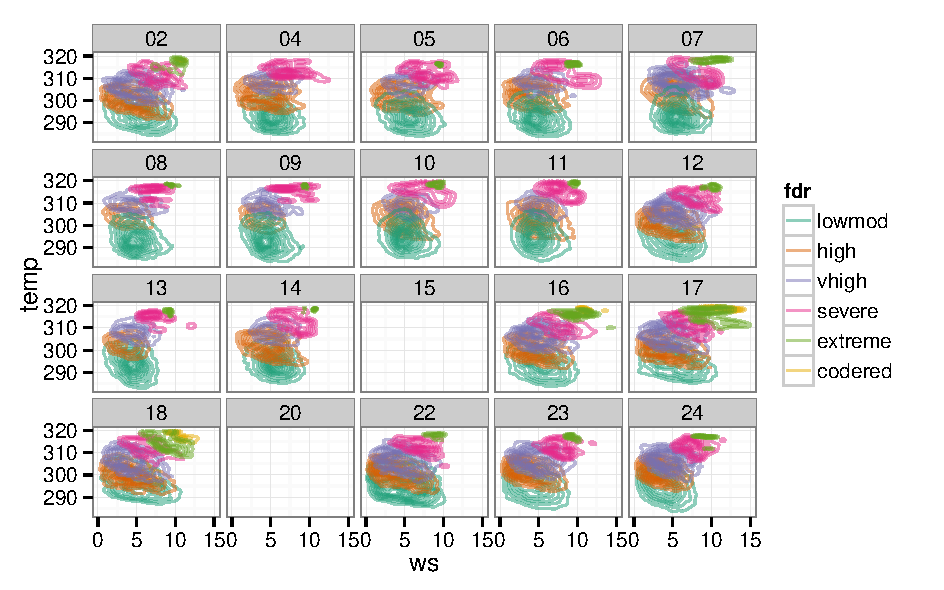
\includegraphics[width=1\columnwidth]{figures/Data/tw_fdr.pdf} 
	\caption{Wind Speed and temperature coloured by fire danger rating} 
	\label{fig:tw_fdr} 
\end{figure}

The FFDI is most sensitive to temperature and windspeed (\cite{dowdy10}). Figure \ref{fig:tw_fdr} shows two-dimensional density plots for windspeed and temperature coloured by the fire danger rating (only observations from October-March included) and divided by CFA district. The relative sizes of each contour show the small proportion of extreme and code red days and the difference in weather conditions observed in different parts of Victoria. For instance the only districts observing code red days are districts 16, 17 and 18. 

The plots for districts 15 and 20 are missing due to there not being enough datapoints in each fire dating rating level to produce the 2D densities.  
 
\subsubsection{Grassland Curing}
The level of dying or senescence of plant material caused by seasonal weather patterns is refered to as grassland curing. Grassland curing ranges between 0 and 100, where 0 means the grass is green with high moisture content and 100 means the grass is at its driest. Curing has a significant impact on fire behaviour in grasslands, particularly the probability of ignition and subsequent rate of spread \citep{cheney08}. 

The grassland curing data were obtained through the Bureau of Meteorology TERN server and AusCover (http://www.auscover.org.au). AusCover is the remote sensing data products facility of the Terrestrial Ecosystem Research network (TERN, http://www.tern.org.au). There are several different satellite models available to provide curing values for image pixels across the state of Victoria. I use `MapVictoria' \citep{martin15} as this is the current algorithm used by the CFA and is shown to outperform the other curing models. 

The curing values are derived from surface reflectance estimates which in turn are derived from cloud-free satellite observations in an 8-day window on a 500-m grid. The dataset spans from the beginning of 2000 to the end of 2010. Missing values may occur in the event of extended cloud cover during the observation window.

Page 10 shows how the level of grassland curing (maximum, minimum and average) changes over each fire season in our sample separated by CFA district. We can see that the districts 2, 5, 8, 16, 17, 18, 20 \&  22 generally dry out faster and have higher minimum curing values relative to districts 4, 6, 9, 10 \& 13. The evolution of grassland curing across the districts clearly demonstrates differing conditions across different parts of the state. 

%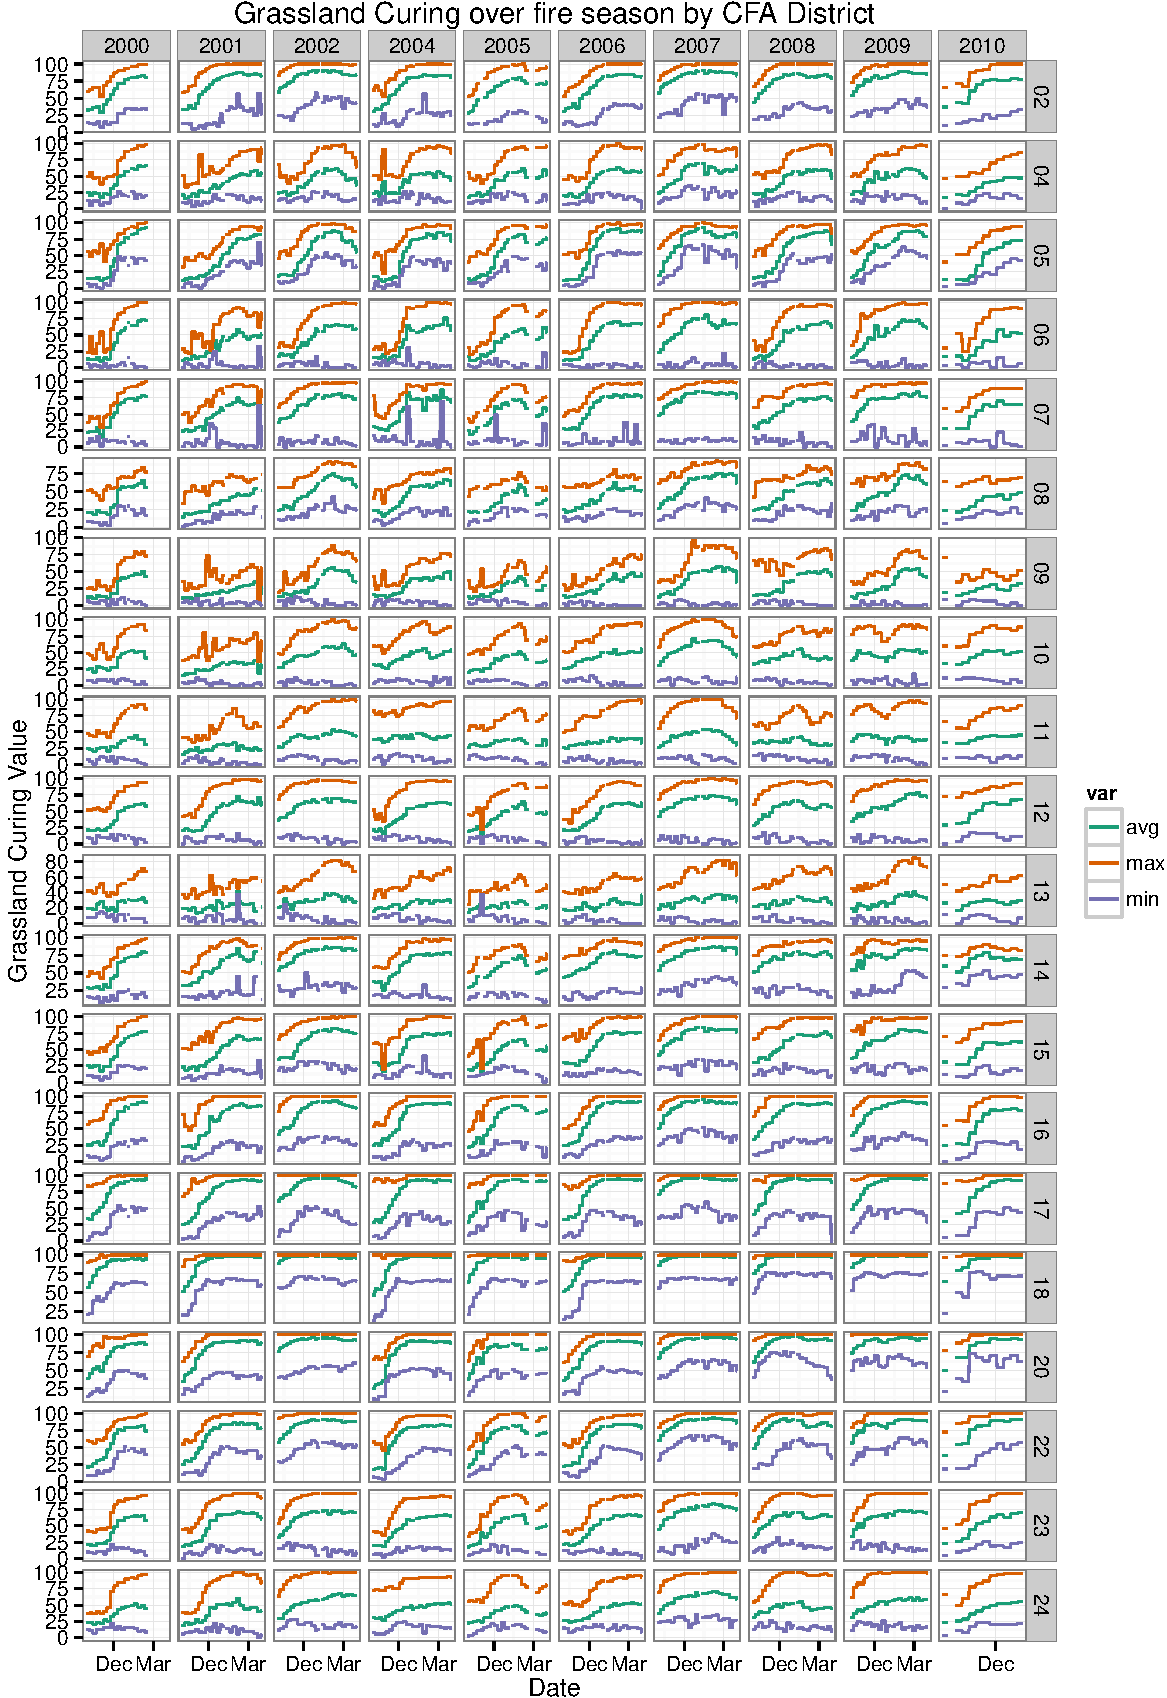
\includepdf[pages={1}]{figures/Data/curdist.pdf}


% level plot of GS curing, probably needs resizing
\begin{figure}[h]
	\centering 
%	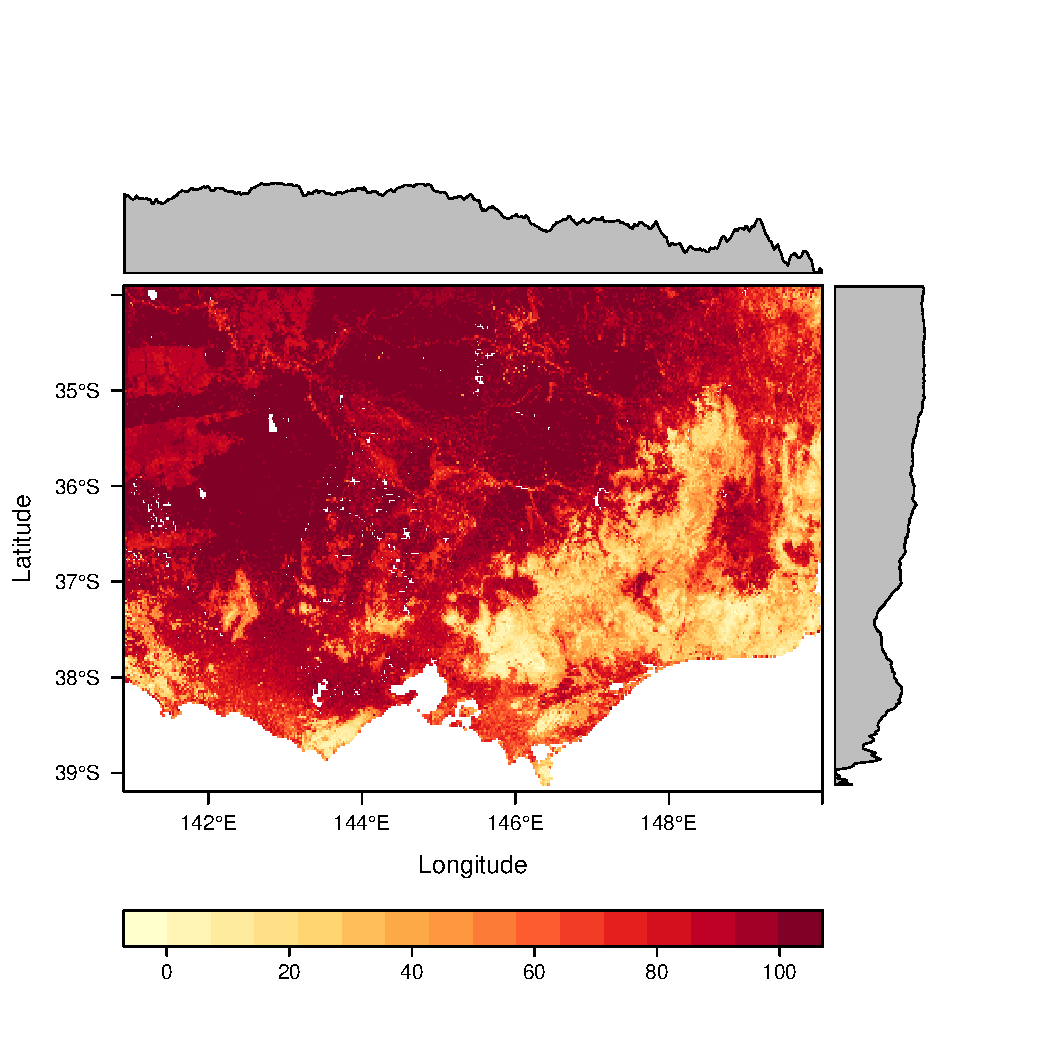
\includegraphics[width=1\columnwidth]{figures/Data/cur_lp.pdf} 
	\caption{Level Plot of Grassland Curing } 
	\label{fig:cur_lp} 
\end{figure}


Figure \ref{fig:cur_lp} shows a level plot produced using the rasterVis package \citep{rastervis}. We observe grassland curing values across the state for the week beginning 25th January 2009. The horizontal margin shows the mean curing value for each longitude and the vertical margin shows the mean curing for each lattitude. The plot clearly shows the difference in curing values across the state, in particular the difference between the east and west of the state. This is consistent with time series graphs of curing. 

\subsubsection{Vapour Pressure}
Vapour pressure, in meteorology, describes the partial pressure of water vapour in the atmosphere, it is directly related to the number of water vapour molecules in the air.  \citet{harris14} find there is a significant relationship between fire activity and vapour pressure among other climate variables. I investigate whether vapour pressure at 9am can improve prediction of fire occurence. 

The vapour pressure dataset was also obtained from the Bureau of Meteorology TERN server and AusCover. The vapour pressure dataset is gridded analyses of daily air water vapour pressure from the Bureau of Meteorology's thermometer network across Australia \citep{jones09}, calculated on a 5km grid. 

% level plot of vapour pressure, level plot may be unnesc could just have std plot
\begin{figure}[h]
	\centering 
%	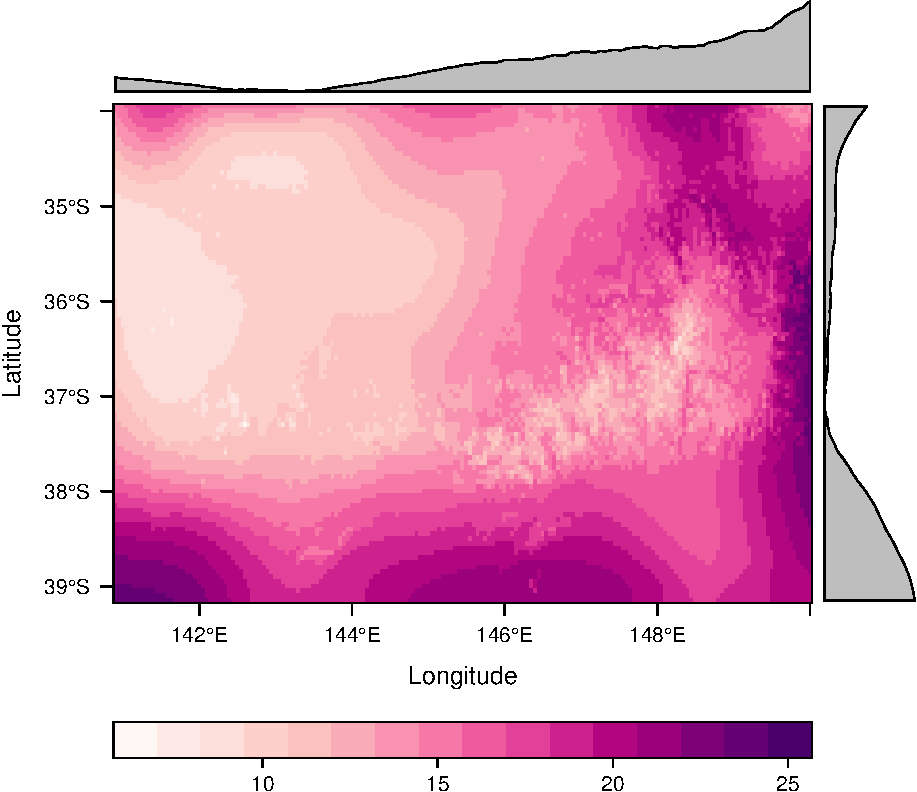
\includegraphics[width=1\columnwidth]{figures/Data/vap_ras.pdf} 
	\caption{Raster plot of vapour pressure 9am } 
	\label{fig:vap_ras} 
\end{figure}

Figure \ref{fig:vap_ras} shows a level plot of the vapour pressure at 9am \citep{rastervis}. The pixel values of the vapour pressure across the state on the 7th of February 2009. We see very clearly in the north-west of the state vapour pressure at 9am is much lower relative to the south-east. 


\subsubsection{Precipitation}

The rainfall data are gridded analyses of daily rainfall measurements from the Bureau of Meteorology's rain gauge network (TERN, AusCover) derived from daily rainfall values from weather stations across Australia. 

The daily rainfall data represents the amount of precipitation of any type observed by means of rain gauges measuring millimeters of liquid water depth over a 24-hour period. The 24-hour period runs from local time 9am the day before to 9am the current day. Rainfall values from sites across the country are analysed onto a 0.05° × 0.05° grid.

\begin{table}[ht]
	\centering
	\begin{tabular}{rrrrrrrrr}
		\hline
		& ffdi & temp & df & rh & ws & curing & rain & vap \\ 
		\hline
		ffdi & 1.00 & 0.77 & 0.62 & -0.77 & 0.04 & 0.51 & -0.20 & 0.01 \\ 
		temp & 0.77 & 1.00 & 0.43 & -0.70 & -0.18 & 0.46 & -0.10 & 0.39 \\ 
		df & 0.62 & 0.43 & 1.00 & -0.58 & -0.09 & 0.47 & -0.37 & -0.08 \\ 
		rh & -0.77 & -0.70 & -0.58 & 1.00 & 0.19 & -0.49 & 0.31 & 0.06 \\ 
		ws & 0.04 & -0.18 & -0.09 & 0.19 & 1.00 & 0.01 & 0.07 & -0.16 \\ 
		curing & 0.51 & 0.46 & 0.47 & -0.49 & 0.01 & 1.00 & -0.11 & 0.05 \\ 
		rain & -0.20 & -0.10 & -0.37 & 0.31 & 0.07 & -0.11 & 1.00 & 0.17 \\ 
		vap & 0.01 & 0.39 & -0.08 & 0.06 & -0.16 & 0.05 & 0.17 & 1.00 \\ 
		\hline
	\end{tabular}
	\caption{Correlation matrix of variables}
	\label{table:correl}
\end{table}

Table \ref{table:correl} shows the cross correlaton matrix for the variables used to predict probability of ignition. High correlation can pose a problem in regression models and to a lesser extent machine learning methods. Variables of concern are temperature, drought factor, relative humidity and FFDI and  which have relatively strong correlation coefficients. 

\subsection{Response Variable: Fire Occurence}

%Commented out until final printing, 
%Map of fire ignitions in Victoria
\begin{figure}[h]
	\centering 
%	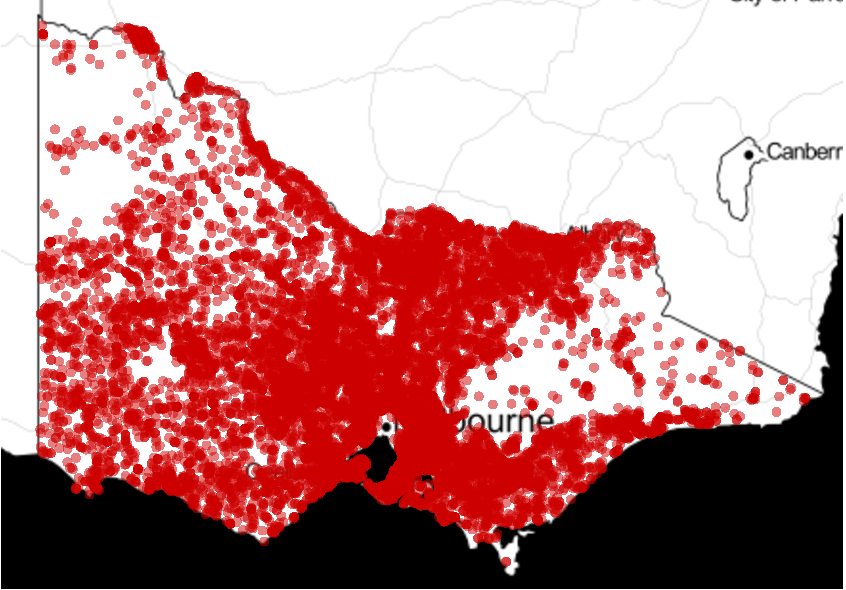
\includegraphics[width=1\columnwidth]{figures/data/firemap.pdf} 
	\caption{Map of fire ignition 2000 - 2009} 
	\label{fig:firemap} 
\end{figure}

%timeseries histogram with count of ignitions per fortnight
\begin{figure}[h]
	\centering 
%	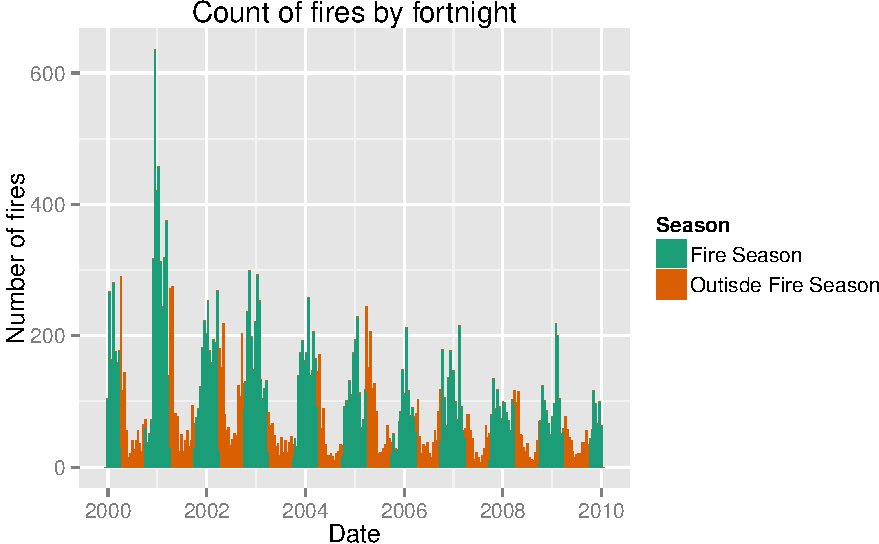
\includegraphics[width=1\columnwidth]{figures/data/occurence.pdf} 
	\caption{Number of ignitions by fortnight} 
	\label{fig:occ} 
\end{figure}

The fire occurrence data comes from the Fire and Incident Reporting System (FIRS). When the Country Fire Authority or other agency attends a fire or other incident a report is prepared and submitted to the FIRS database. The FIRS dataset used in this study includes all grass, grass and scrub, forest and bushfire in Victoria from the beginning of the year 2000 to 2014. 

Recent work by the Bushfire and Natural Hazards Cooperative Research Centre integrating bushfire and planned burn datasets in Victoria give an indication on the reliability of the data (Kilinc et al. 2015).  There is significant uncertainty of accuracy of the fire size, in particular for smaller scale fires. To limit the impact of this imperfection the data is transformed into a binary response variable where a 1 denotes a fire and a 0 denotes no fire. 

The data also contains some approximate coordinates for the point of origin for fires, however as discussed below the data is aggregated to a 10km grid. Consequently small errors in the fire coordinates are not deemed to cause a problem. 

Figure \ref{fig:firemap} shows the locations of the fires in the dataset on the map of Victoria. The most noticable thing in Figure \ref{fig:firemap} is the sparsity of fires in the north-east and north west of the state and around Melbourne. This is due to the division of fire fighting organisations in Victoria. The sparse areas correspond to National Parks where Parks Victoria or the Department of Environment, Land, Water and Planning (DELWP) coordinate fire fighting activities, so many of the fires occuring in these areas are not included in this dataset. 




\begin{figure}[h]
	\centering 
%	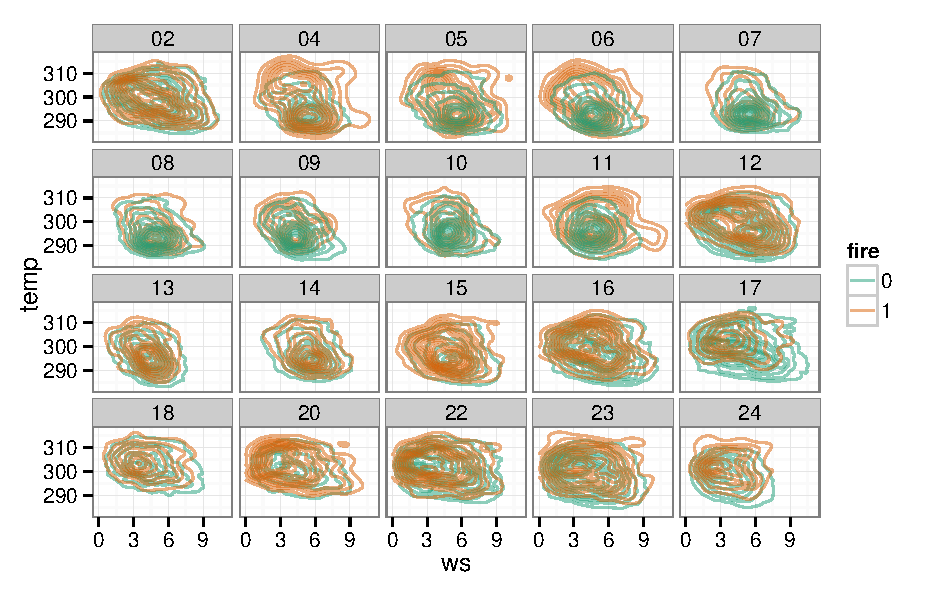
\includegraphics[width=1\columnwidth]{figures/Data/tw_fire.pdf} 
	\caption{Wind Speed and temperature coloured by fire/no fire} 
	\label{fig:tw_fire} 
\end{figure}

Figure \ref{fig:tw_fire} is constructed in the same manner as Figure \ref{fig:tw_fdr} but instead of grouping by the fire dange rating, I group by Fire/No Fire. Windspeed and temperature play the largest role in determining the FFDI yet there is no discernable difference between the distributions of the two variables when there is a fire compared to no fires. This is the first indicator that the FFDI alone may not be a good predictor of probability of ignition. 

\begin{figure}[h]
	\centering 
%	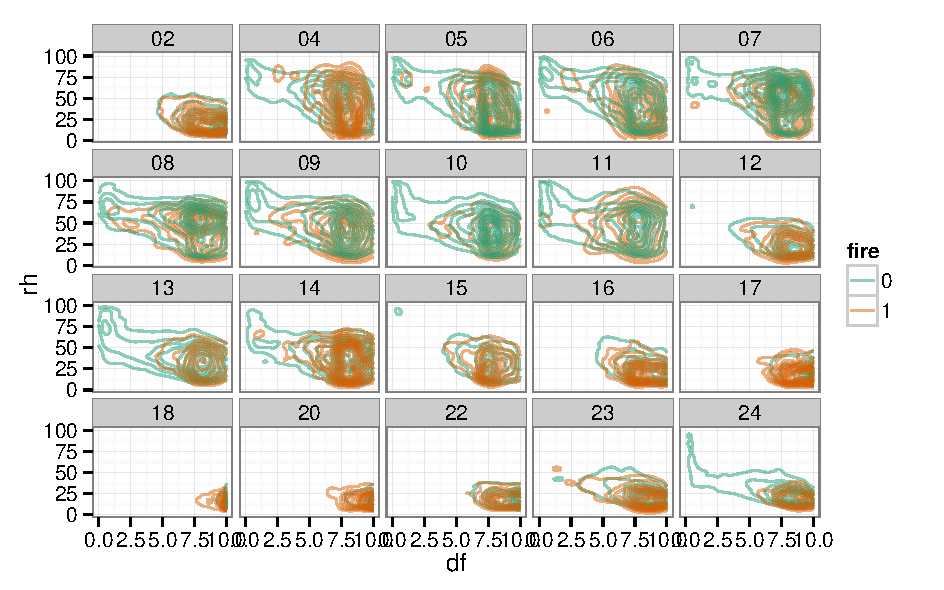
\includegraphics[width=1\columnwidth]{figures/Data/dh_fire.pdf} 
	\caption{Drought factor and relative humidity coloured by fire/no fire} 
	\label{fig:dh_fire} 
\end{figure}

Plotting the 2D densities of the drought factor and relative humidity in Figure \ref{fig:dh_fire}, ranges of relative humidty don't appear to vary on fire days compared to not fire days but in districts 4, 5, 6, 7, 8, 9, 10, 11, 13, 14 and 24 there is a clear difference in the densities of fire compared to no fire. Small drought factors are mostly associated with non-fire days. In districts 2, 12, 15, 16, 17, 18, 20 and 22 do not have large differences in the two densities, these districts generally have high drought factor and low relative humidity. 

\begin{figure}[h]
	\centering 
%	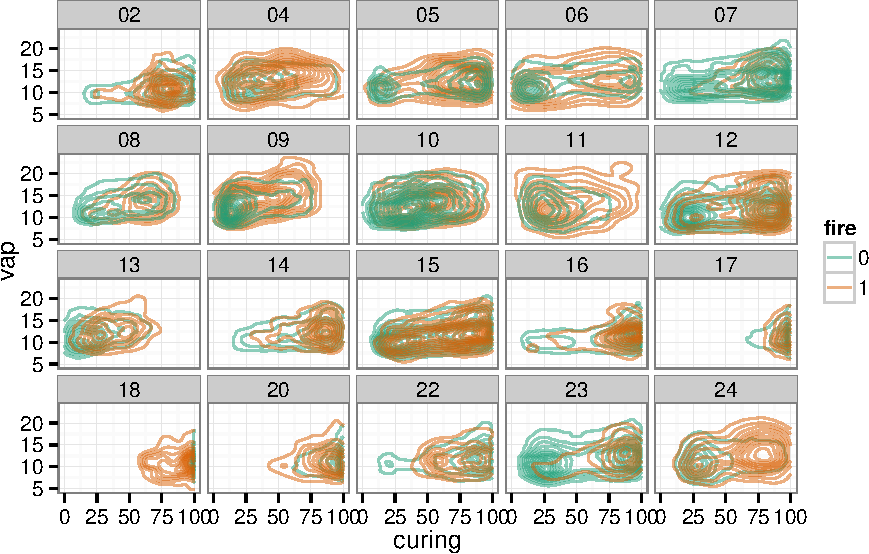
\includegraphics[width=1\columnwidth]{figures/Data/gv_fire.pdf} 
	\caption{Grassland curing and vapour pressure coloured by fire/no fire} 
	\label{fig:gv_fire} 
\end{figure}

In Figure \ref{fig:gv_fire} shows the 2D densities for grassland curing and vapour pressure for the fire and non-fire days. Once again we see a clear difference in behaviour across districts.  

\subsection{Assembling datasets}

Assembling the datasets began with the meterological data from the WRF model. This data came in NetCDF form \citep{ncdf}. The dataset spanned all of Eastern Australian (Queensland, New South Wales \& Victoria) with daily observations over a 25 year period. This area, divided into 10km grids, contained 28675 gridpoints each of which had longitude, lattitude and weather variable values (temperature, wind speed, relative humidty, FFDI and drought factor) associated with it. Once the time component is taken into account, the original dataset contained over 200 million data points ($28675 \times 365 \times 25$). 

The first step was to reduce the dataset to a more manageable size. I converted the NCDF file to a datatable using the raster and data.table packages in R \citep{raster, datatable}. I used ESRI shapefiles of Australian Geographical Classification boundaries \citep{ABS1259} to sort the gridpoints into states and selected only gridpoints in Victoria. The datasets intersect between 2000 and 2009, subsetting the WFR data reduces the size of the dataset to just over 8 million data points. 

From Figure \ref{fig:occ} it is clear the majority of bushfires occur during the fire season. I reduce the size of the dataset, taking only observations in Victorian fire season (October to March) for a number of reasons. First, from a policy perspective the FFDI, fire danger rating systems, grassland curing are only calculated during the fire season so using these variables outside the time periods they are available does not make intuitive sense. From a practical perspective, this paper is looking at predicting the types bushfires that threaten lives and property which we know to occur in the summer months. 

Classification trees and random forests are computationally intensive. Only using the fire season reduces the dataset to just over 3 million observations, significantly reducing computation time without compromising the project. 

From the fire occurence dataset this study used the date and coordinates of the fire. The coordinates were given in the Australian Map Grid (AMG66), a coordinate reference system derived from a Universal Transverse Mercator(UMT) projection of latitudes and longitudes on the Australian Geodetic Datum (AGD) \citep{featherstone96}. To merge the meterological data set and the fire occurence dataset I needed to convert from this UMT projection to longitude and lattitude using the sp package in R \citep{sp08}. 

Once the coordinates of fires were converted to the same projection I matched each fire coordinate to its nearest neighbour from the meterological dataset. Once matched it was straightforward to merge the two datasets based on grid point and date \citep{datatable}. 

The different CFA districts and regions were added into the dataset using the raster package and another ESRI shapefile containing the district boundaries \citep{raster}. 
Digital boundaries for the CFA area compared to MFB or DELWP response areas were unavailable, as such an alternate method to subset geographical area was used. I made the assumption that if the CFA had not attended a bushfire betwen 2000 and 2014 within a 5km region of the gridpoint, then the gridpoint was unlikely to be in a CFA area. Accordingly any grids that had no fire occur in them since 2000 were excluded from the dataset. 

The three additional variables (grassland curing, vapour pressure and precipitation) came as raster files each of higher resolutions than the original 10km grid. In all three sets we have some missing values or faulty readings due to technological fault. To minimise the impact of these for each for each gridpoint in the meteorological dataset I find the pixels contained in each gridpoint and take the median value for each time period. The functionality to combine spatial points and raster layers is provided by the raster package \citep{raster}. For any remaining missing values I make the assumption that cloud cover or faulty barometer readings are sufficiently random such that missing values will not bias results.
 
%In addition to differing spatial resolutions, the grassland curing dataset has a different timescale resolution. Curing is recorded every 8 days, while the rest of the dataset is on a daily scale. As a result the grassland curing value holds 

This final dataset is divided into a testing (30\%) and training set (70\%) randomly sampling across 'Fire' and 'No Fire' such that both datasets have the same proportion of 'Fire' (approximately 0.05). 

\section{Method}

\subsection{Logistic regression}

Use of logistic models is the usual method for dealing with a binary response problem and it is common in studies on fire occurrence or ignition.  In this project I use logistic regression models and in addition to the linear constructions used in \citet{andrews03} and \citet{del11} I take into account the non-linear relationship believed to exist between the explanatory variables and dependent variable through the inclusion of regression splines. 

Regression splines are a method for modelling nonlinear data as a number of piecewise  polynomial functions. The points at which the functions join are called knots. For example when the functions join at $x=k$, $k$ is known as a knot \citep{ruppert03}.

As a result the logistic model becomes
\begin{equation}
\label{eq logits}
\Pr(Y=1|X)=\frac{\exp(\sum_{k=1}^K f_k(x_k))}{1+\exp(\sum_{k=1}^K f_k(x_k)}
\end{equation}
where $Y$ denomtes fire occurence, $x_k$ denotes the $k$th predictor and each $f_k$ represents a penalized regression spline.

Regression splines can be subject to over fitting: where the fitted model adheres to the data too strongly and doesn't smooth out `noise' enough. This results in great in-sample predictions but poor out-of-sample predictions. To prevent over fitting occurring we use an automated method that optimizes the number of knots by penalizing for non-smoothness; an overview of using penalized regression splines in this context is given by \citet{wood02}. 

\subsection{Classification trees}

Classification tree analysis involves segmenting the predictor space into different regions in order to find the best predictor for the response variable. 

The task of finding the single best predictor is achieved using recursive partitioning of the data and can be summarized as two major steps:
\begin{enumerate}
	\item For each predictor multiple cut points are evaluated and the quality of the split is based on the Gini index. Equation (\ref{eq gini}) gives the Gini index for a binary variable:
	\begin{equation}
	\label{eq gini}
	G=\sum_{k=1}^{K} \hat{p}_{mk} (1-\hat{p}_{mk})
	\end{equation}
	where $\hat{p}$ is the estimated probability of a fire at that node. It is also possible to use the cross entropy \citep{james13} which like the Gini index takes on a small value if the node is pure. 
	For each predictor the best cut point is chosen. 
	\item The best split overall is chosen:  For each predictor and its corresponding ‘best’ split, the overall best split is chosen again based on Gini index. 
\end{enumerate}

The best split for the best predictor defines the first two subsets then same two step procedure is applied to each partition separately and repeated with all subsequent partitions until there is no meaningful reduction in the Gini index \citep{berk08,james13}. 

Decision tree analysis results in a model which is simple to explain, interpret and represent graphically \citep{james13}. This is particularly advantageous in the context of fire danger rating systems.
This decision tree is expected to perform well relative to the logistic model as in this situation we expect a simple formula like equation (\ref{eq logits}) to be inadequate in representing the relationship between the predictors and the response variable.  

Two common problems associated with decision trees are the problem of overly complex trees (or over fitting) and secondly that in the quest to reduce the Gini index it is possible to subdivide the data so far that there are very few observations at each node. 

To approach over fitting, one of two different approaches can be taken: either a rule can be applied that prevents the tree growing too large (for example by setting a threshold on the minimum amount of information gain required to produce a split), or the tree can be allowed to grow large and pruning can be applied afterwards to produce a subtree. In this paper I use 10-fold cross validation on the training data to choose the precision parameter for the classification tree. 

Decision trees tend to be very sensitive to the sample used to grow them. Taking this into account I build a number of trees using different balanced samples of the data and compare the output. An alternative solution is random forests (discussed below) as they have the additional advantage of reducing the problem of high variance which plagues decision trees \citep{james13}. 

In interpreting classification trees, proximity to the base of the tree indicates how important the variable is in predicting fire occurrence. Variables at the base of the tree are the most important. A tree which does not have the FFDI close to the base of the tree this will suggest the FFDI is not the most important predictor for fire occurrence. Using those variables close to the base of the tree in a fire danger rating system should improve its predictive ability. 



\subsection{Random forests}

A random forest is a technique that uses classification trees as a key building block and helps address the limitations of classification trees and improve predictive performance. They involve multiple trees and random samples of our predictors \citep{berk08}. 
The general algorithm is as follows for our dataset of N observations and P predictor variables \citep{berk08, varian14}:

\begin{enumerate}
	\item Take a bootstrap sample (random sample of size N with replacement) from the data. 
	\item Take a random sample of size $M \textless P$ (typically $M \approx \sqrt{P}$, \cite{james13}, without replacement) from the predictors. 
	\item Construct a classification tree using these samples of data and predictors.
	\item Repeat from step 2 for each subsequent split until the tree is as large as desired. Do not prune. 
	\item Drop observations not included in the bootstrap sample from step 1 (known as out-of-bag data) down the tree. The class assigned to each observation is stored along with each observations predictor values.
	\item Repeat steps 1-5 a large number of times to grow a forest of trees. 
	\item In order to determine the classification of a new observation. Have each tree make a classification and use a majority vote for the final prediction.
\end{enumerate}

As discussed above, decision trees suffer from high variance. Taking an average of a set of predictions, as we do in random forests, reduces the variance of the predicted values. The second step of the Random Forests algorithm is an integral part of the reducing variance. By taking a sample of M predictors some of the trees will not have a chance to consider the strongest predictors allowing other predictors to add some value and results in less correlated predictions. Averaging many uncorrelated predictions has a greater reduction in variance than averaging many correlated predictions, thus the average prediction for the random forests will be less variable and more reliable \citep{james13}.

The repeated splitting based on parameters by the random forest allows the forest to detect interaction effects between variables. The definition of interaction used for random forests is that two variables interact if a split on one variable in a tree makes a split on the other variable either systematically less possible or more possible \citep{breiman01}. Detection of interactions is based on the gini values,  details of various methods given by \citet{kelly12}. The ability of the forest to detect interaction automatically is a key advantage of the forest over models such as logistic regression where the researcher must specify any interaction terms. 
%Klaus: Random forest: one thing you should add is the interaction detection. The repeated splitting based on parameters help the random forest to detect interaction terms in a way automatically. This is a big advantage over logistic regression where you have to specify themselves. The drawback is though, that it does not tell you what the interaction terms are.
% Brieman: The operating definition of interaction used is that variables m and k interact if a split on one variable, say m, in a tree makes a split on k either systematically less possible or more possible. The implementation used is based on the gini values g(m) for each tree in the forest. These are ranked for each tree and for each two variables, the absolute difference of their ranks are averaged over all trees.

Some of the weaknesses of Random Forests is that they can be a ‘black box’ in that it is difficult to understand where the output is coming from and they do not offer simple summaries of the relationship between variables in the way decision trees do \citep{varian14}. The advantages of decreased variance and improved accuracy of predictions which random forests bring come at the cost of interpretability, random forests cannot be represented in a clear diagram and it is no longer immediately obvious which variables are the most influential in the procedure \citep{james13}. 

I expect the random forest model to give improved out-of-sample fit particularly with highly non-linear data and despite being difficult to interpret, the random forests can offer insight regarding which predictors contribute the biggest improvements to prediction accuracy \citep{varian14}.


\subsection{Classification with unbalanced classes}

Classical machine learning algorithms assume that the response variable has an equal number of observations within each class. Classes are considered imbalanced if the proportion of observations in one class is not equal to the proportion of observations in the other \citep{japkowicz00}. In practice it is very common to have some degree of imbalance and this does not have much effect on the outcome unless the imbalance reaches some threshold. 

In the context of fire occurence, even during the fire season in Victoria instances of bushfire are not that common. For any given day in the dataset at most 4.5\% of the grids experience fire, some days it is possible to have no fires at all. Intuitively, before looking at the data we can expect the proportion of fire days is much smaller than that of non fire days. 

Restricting the dataset to the Victorian fire season (October to March) marginally improves the imbalance problem; nevertheless the proportion of fire days of total days for each spatial point is 0.0053. It is safe to say that this situation is one where the degree of imbalance is problematic as a classifier which always assumes `no fire' has an expected error rate of 0.5\% leaving very little room for a more complicated classifer to improve upon. 

There are several ways to address the class imbalance problem in machine learning: over sampling, undersampling, using different splitting criteria \citep{japkowicz00}. 

I address the class imbalance problem in two ways, first in building the model I create balanced samples by under sampling the `no fire' class in a similar manner to \citep{padilla11}.  The second approach is to assess each model's performance in predicting the test data using 'balanced accuracy' rather than overall accuracy \citep{mosley13, japkowicz00}. 

Undersampling the no fire class addresses the problem of imbalanced classes but I also use it to reduce the serial and spatial correlation that is present in the dataset by using a ~near-maximin' sampling method thereby ensuring all the datapoints in the sample are separate from each from each other in space and time to reduce the impact of correlation. 

For consistency all three of the classification techniques are estimated on the balanced training set and evaluated by  on the test data. I evaluate based on receiver operating characteristic (ROC) plots  and using 2 x 2 confusion matrices. 

An example confusion matrix is given in table \ref{table:ex}. 
%eg confusion matrix with ABCD
\begin{table}[ht]
	\centering
	\begin{tabular}{r|rr|r}
		& Model & & \\ 
		\hline
		& Prediction   & &  \\ 
		Reference & No Fire & Fire & \\ 
		\hline
		No Fire & a & a & a+b \\ 
		Fire & c & d  & c + d \\ 
		\hline
		 & a+c & b+d & N \\
	\end{tabular}
	\caption{Example confusion matrix}
	\label{table:ex}
\end{table}

Accuracy is defined as:
\begin{equation}
\label{eq acc}
\mbox{Accuracy} = \frac{a + d}{a+b+c+d}
\end{equation}

I also report sensitivity (correctly classified fires dividied by total number of actual fires) and specificity (correctly identified non-fires divided by total number of non-fires), balanced accuracy and kappa. 

\begin{equation}
\label{eq sens}
\mbox{Sensitivity} = \frac{a }{a+b}
\end{equation}

\begin{equation}
\label{eq spec}
\mbox{Specificity} = \frac{d}{c+d}
\end{equation}


\begin{equation}
\label{eq BA}
\mbox{Balanced Accuracy} = \frac{\frac{a }{a+b} + \frac{d}{c+d} }{2}
\end{equation}


\begin{equation}
\label{eq:K}
\kappa = \frac{P_0 - P_c}{1-P_c}
\end{equation}

where $P_0$ is the total agreement probability and $P_c$ is the “agreement” probability which is due to chance ( see \cite{kappa} for definitions )

On top of the accuracy measures in equations (\ref{eq sens}), (\ref{eq spec}) and (\ref{eq BA}) the value in the bottom left of the confusion matrix (c) where we incorrectly predict ~No fire' is very important in this context. 

 As a secondary measure of model quality, I use ROC plots as they remove the requirement of assuming a cut-off value. 

An ROC plot shows the change in true positive rate (sensitivity) and false positive rate (1- specificity) for different probability thresholds. For each model I plot the ROC and calculate the area under the curve (AUC) as a measure of the model performance. The AUC measures a classification model's performance, ranging from 0.5 (random) to 1 (perfect accuracy). 

%Also available is a test of significance on the out-of-sample predictions known as McNemar's test \citep{dietterich98}. 


\section{Results}

\subsection{Logistic Regression}

The baseline model is given by a simple logistic regression of fire on FFDI, I then add the inputs to the FFDI and  the other variables (curing, vapour pressure and rainfall). 

Logistic regression output for the first three models is given in table \ref{table:coefficients}. 

The signs of the coefficients for the input variables are as we would expect: temperature, windspeed, drought factor and curing have a positive effect on probability of ignition while relative humidity and rain have a negative effect. 

%**Vapour pressure sign on pr ignition sarah finds below average vapour pressure correlated with fire activity while the sign on vapour pressure in the regression is positive. *serial correlation?

The coefficient on FFDI is positive in model 1 but on including other variables the  sign changes to negative. This is very difficult to interpret as it is impossible to hold all the input  variables constant and increase the FFDI so it cannot be interpreted alone. 

The coefficient on vapour pressure is of concern, previous studies on fire activity including vapour pressure \citep{harris14} found below average vapour pressure is correlated with fire activity which leads us to expect a negative coefficient. The regression reports a positive and statistically significant coefficient. 
%(This may be because Sarah's study only looked at linear correlation and vapour pressure will be correlated with rainfall, so HAEC vapour pressure actually does have a positive impact on fire activity maybe it is connected with storms? )

Individual t-statistics indicate even when FFDI is taken into account it's inputs are still statistically significant in determining probability of fire. 
%(Although this may just be becuase the sample size is very large). 

A likelihood ratio test rejects the null that temperature, relative humidity, windspeed and drought factor are jointly insignificant providing further evidence that the FFDI is not using the meteorological information efficiently and there are relationships between fire occurence and these variables that the FFDI is not capturing.

%Do I need to show output for this? 

With the addition of our other meteorological variables in the logistic Model 3, the P-values once again suggest that rain and vapour pressure at 9am are statistically significant but grassland curing is not statistically significant at the 5\% level. The statistical significance of rainfall and vapour pressure suggest more could be added to the index to produce a better prediction of fire occurrence. 

%**How to do LR test on diff num observations? 
% Table: Regression output
\begin{table}
	\begin{center}
		\begin{tabular}{l c c c }
			\hline
			& Model 1 & Model 2 & Model 3 \\
		\hline
		(Intercept)    & $-0.1050^{***}$ & $-18.2314^{***}$ & $-15.4002^{***}$ \\
		& $(0.0204)$      & $(1.0391)$       & $(1.4012)$       \\
		ffdi           & $0.0073^{***}$  & $-0.0423^{***}$  & $-0.0370^{***}$  \\
		& $(0.0011)$      & $(0.0025)$       & $(0.0028)$       \\
		temp           &                 & $0.0604^{***}$   & $0.0504^{***}$   \\
		&                 & $(0.0034)$       & $(0.0048)$       \\
		rh             &                 & $-0.0100^{***}$  & $-0.0103^{***}$  \\
		&                 & $(0.0013)$       & $(0.0015)$       \\
		ws             &                 & $0.0666^{***}$   & $0.0687^{***}$   \\
		&                 & $(0.0074)$       & $(0.0082)$       \\
		df             &                 & $0.1084^{***}$   & $0.0682^{***}$   \\
		&                 & $(0.0072)$       & $(0.0084)$       \\
		curing         &                 &                  & $0.0012$         \\
		&                 &                  & $(0.0006)$       \\
		rain           &                 &                  & $-0.0525^{***}$  \\
		&                 &                  & $(0.0057)$       \\
		vap            &                 &                  & $0.0244^{***}$   \\
		&                 &                  & $(0.0062)$       \\
		\hline
		AIC            & 31809.3877      & 31229.3462       & 26589.0141       \\
		BIC            & 31825.4721      & 31277.5994       & 26659.9683       \\
		Log Likelihood & -15902.6938     & -15608.6731      & -13285.5071      \\
		Deviance       & 31805.3877      & 31217.3462       & 26571.0141       \\
		Num. obs.      & 22976           & 22976            & 19610            \\
		\hline
		\multicolumn{4}{l}{\scriptsize{$^{***}p<0.001$, $^{**}p<0.01$, $^*p<0.05$}}
	\end{tabular}
	\caption{Logistic regressions output}
	\label{table:coefficients}
\end{center}
\end{table}

I add splines to Model 3 in stages using the confusion matrices for 10-fold cross validation to assess accuracy (using the caret package by \cite{caret}). The best performing model based on balanced accuracy and number of false negatives (incorrectly predicted ~No Fires') is reported in table \ref{table:logf}. 

Interestingly, in Model 3 grassland curing is not statistically significant while all the other variables in the model are significant at 0.1\% level. Once the splines are added to the model, the FFDI function, wind speed, and vapour pressure are no longer significant but grassland curing is statistically significant. 

Figure \ref{fig:gam_pl} shows the spline functions for each of the inputs. In logistic models the spline functions are not the marginal effects of the variables on probability of ignition but the marginal effect on the log-odds ratio. Equation \ref{eq logits} can be rearranged to give equation \ref{eq:logodds}, the log-odds ratio \citep{james13}. 

\begin{equation}
\label{eq:logodds}
\log(\frac{p(X)}{1-p(X)}) = \sum_{k=1}^{K} f_k (x_k)
\end{equation}

The spline function fitted on the FFDI although non-linear, according to the standard error is not statistically different from zero (also seen in the p-values in table \ref{table:logf}). After taking into account the other variables in the model, FFDI does not appear to have an impact on the log-odds ratio. This may be because the other variables in the model take into account any information contained in the FFDI. 

The drought factor has an almost linear impact on the log-odds ratio when it is inbetween 0 and 6. When drought factor is between 0 and 6 it has a negative effect on log-odds but at a decreasing rate. When the drought factor it between 6 and 9 it has a positive impact on the log-odds ratio, after 9 the effect because negative again. 

Relative humidty appears to have a quadratic relationship with the log-odds ratio. Relative humity only has positive effect on the log-odds ration when it is inbetween 30 and 70\%. This function makes sense intuitively as when relative humidty is very high there is too much moisture in the air (or it is raining) preventing ignition. When relative humidity is very low it does not appear to have a statistically significant impact on the log-odd ratio. The middle values for relative humidty would correspond to warm, dry days, ideal ignition conditions. 

Grassland curing exhibits a right skewed function, having a positive effect on the log-odds ratio between 40 and 95. This behaviour is not as intuitive as relative humidity. Fire science would suggest drier fuel would increase probability of ignition. 

%Output from best performing splines model (used xtable rather than texreg, too inconsistent?)
\begin{table}[ht]
	\centering
	\begin{tabular}{rrrrr}
		\hline
		& Estimate & Std. Error & z value & Pr($>$$|$z$|$) \\ 
		\hline
		(Intercept) & -3.1484 & 0.2757 & -11.4210 & 0.0000 \\ 
		ns(ffdi, 5)1 & -0.2905 & 0.3613 & -0.8043 & 0.4213 \\ 
		ns(ffdi, 5)2 & -0.2304 & 0.4625 & -0.4982 & 0.6183 \\ 
		ns(ffdi, 5)3 & 0.4040 & 0.5589 & 0.7229 & 0.4697 \\ 
		ns(ffdi, 5)4 & -0.4340 & 0.9674 & -0.4487 & 0.6537 \\ 
		ns(ffdi, 5)5 & -0.8815 & 0.7271 & -1.2124 & 0.2254 \\ 
		ns(temp, 1) & 1.8543 & 0.3416 & 5.4276 & 0.0000 \\ 
		ns(rh, 2)1 & 0.9325 & 0.5687 & 1.6397 & 0.1011 \\ 
		ns(rh, 2)2 & -0.6173 & 0.3607 & -1.7115 & 0.0870 \\ 
		ws & -0.0169 & 0.0146 & -1.1541 & 0.2485 \\ 
		ns(df, 5)1 & 1.1093 & 0.2798 & 3.9639 & 0.0001 \\ 
		ns(df, 5)2 & 1.0156 & 0.3115 & 3.2601 & 0.0011 \\ 
		ns(df, 5)3 & 0.7113 & 0.2604 & 2.7319 & 0.0063 \\ 
		ns(df, 5)4 & 0.8071 & 0.5479 & 1.4730 & 0.1408 \\ 
		ns(df, 5)5 & -0.1512 & 0.1950 & -0.7752 & 0.4382 \\ 
		ns(curing, 6)1 & 1.5648 & 0.1388 & 11.2754 & 0.0000 \\ 
		ns(curing, 6)2 & 2.3986 & 0.1874 & 12.7997 & 0.0000 \\ 
		ns(curing, 6)3 & 1.6637 & 0.1640 & 10.1436 & 0.0000 \\ 
		ns(curing, 6)4 & 1.6949 & 0.1335 & 12.6921 & 0.0000 \\ 
		ns(curing, 6)5 & 1.4634 & 0.3436 & 4.2588 & 0.0000 \\ 
		ns(curing, 6)6 & -0.4909 & 0.0817 & -6.0066 & 0.0000 \\ 
		rain & -0.0286 & 0.0056 & -5.0703 & 0.0000 \\ 
		vap & -0.0003 & 0.0067 & -0.0504 & 0.9598 \\ 
		\hline
	\end{tabular}
	\caption{Regression output for Model 4}
	\label{table:logf}
\end{table}

%GAM plots, not sure if this is exactly splines... 
\begin{figure}[h]
\null\vfill\noindent
%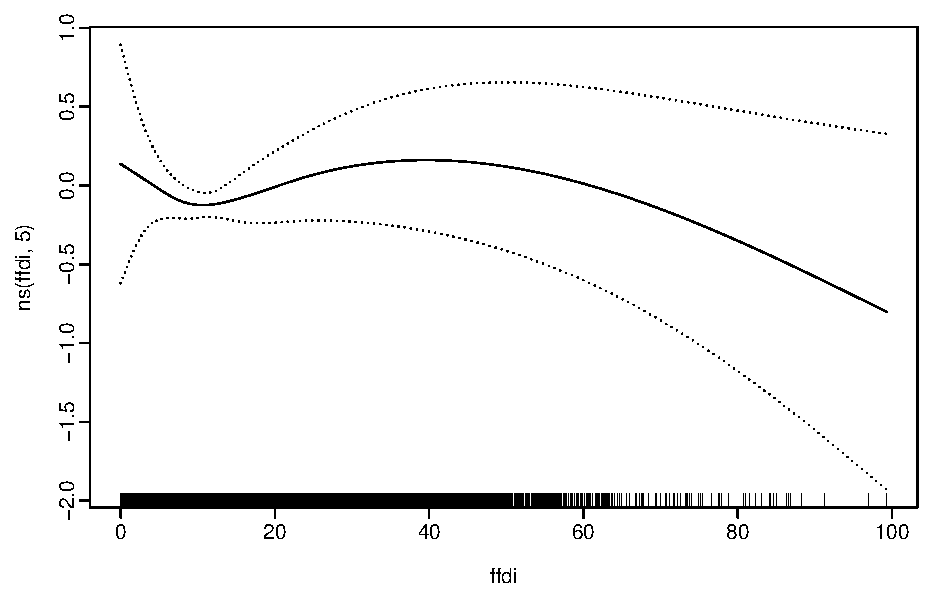
\includegraphics[page=1,width=.48\linewidth,height=.45\textheight,keepaspectratio]{figures/gam_pl.pdf}
\hfill
%\includegraphics[page=2,width=.48\linewidth,height=.45\textheight,keepaspectratio]{figures/gam_pl.pdf}
\vfill
%\includegraphics[page=3,width=.48\linewidth,height=.45\textheight,keepaspectratio]{figures/gam_pl.pdf}
\hfill
%\includegraphics[page=4,width=.48\linewidth,height=.45\textheight,keepaspectratio]{figures/gam_pl.pdf}
\vfill
%\includegraphics[page=5,width=.48\linewidth,height=.45\textheight,keepaspectratio]{figures/gam_pl.pdf}
\hfill
%\includegraphics[page=6,width=.48\linewidth,height=.45\textheight,keepaspectratio]{figures/gam_pl.pdf}
\vfill
\null
	\caption{Plots of smoothing functions in Model 4 with 95\% pointwise confident interval} 
	\label{fig:gam_pl} 
\end{figure}

The focus of this project is to build an accurate predictor of fire ignition, so out of sample prediction is a more important evaluation tool than hypothesis testing. Table \ref{table:cm2} contains confusion matrices (values are proportions of total number of observations in the test set) based on test data predictions, using a cutoff value of 0.5. The confusion matrix is accompanied by measures of accuracy in table \ref{table:acc2}. 

%Confusion matrix cutoff=0.5
\begin{table}[ht]
	\centering
	\begin{tabular}{r|rr|rr|rr|rr}
		\hline
		& Model 1 &  & Model 2 &  & Model 3 &  & Model 4 & \\ 
		\hline
		& Actual   &  &  &  &  & & & \\ 
		Predict & No Fire & Fire & No Fire & Fire & No Fire & Fire & No Fire & Fire\\ 
		\hline
No Fire & 0.5959 & 0.0030 & 0.4457 & 0.0019 & 0.5111 & 0.0021 & 0.5807 & 0.0016 \\ 
Fire & 0.3989 & 0.0022 & 0.5490 & 0.0034 & 0.4838 & 0.0030 & 0.4142 & 0.0035 \\ 
		\hline
	\end{tabular}
	\caption{Confusion Matrices for Models 1, 2 \& 3 cutoff value 0.5}
	\label{table:cm2}
\end{table}



% Accuracy for cutoff 0.5
\begin{table}[ht]
	\centering
	\begin{tabular}{rrrrr}
		\hline
		& 1 & 2 & 3 & 4 \\ 
		\hline
Sensitivity & 0.5990 & 0.4481 & 0.5137 & 0.5837 \\ 
Specificity & 0.4267 & 0.6476 & 0.5854 & 0.6920 \\ 
Balanced Accuracy & 0.5129 & 0.5479 & 0.5495 & 0.6378 \\ 
Accuracy & 0.5981 & 0.4492 & 0.5141 & 0.5842 \\ 
Kappa & 0.0007 & 0.0018 & 0.0021 & 0.0067 \\
		\hline
	\end{tabular}
		\caption{Accuracy for Models 1, 2, 3 \& 4 cutoff value 0.5}
		\label{table:acc2}
\end{table}

Table \ref{table:acc2} shows the gain in balanced accuracy from including both the inputs to the FFDI and the additional variables. The balanced accuracy suggests the inclusion of grassland curing, vapour pressure and rainfall only gives a very marginal improvement while the inclusion of splines yields a larger improvement in balanced accuracy. Clearly the logistic model with regression splines performs the best based on the confusion matrix.

%ROC for logits
\begin{figure}[h]
	\centering 
%	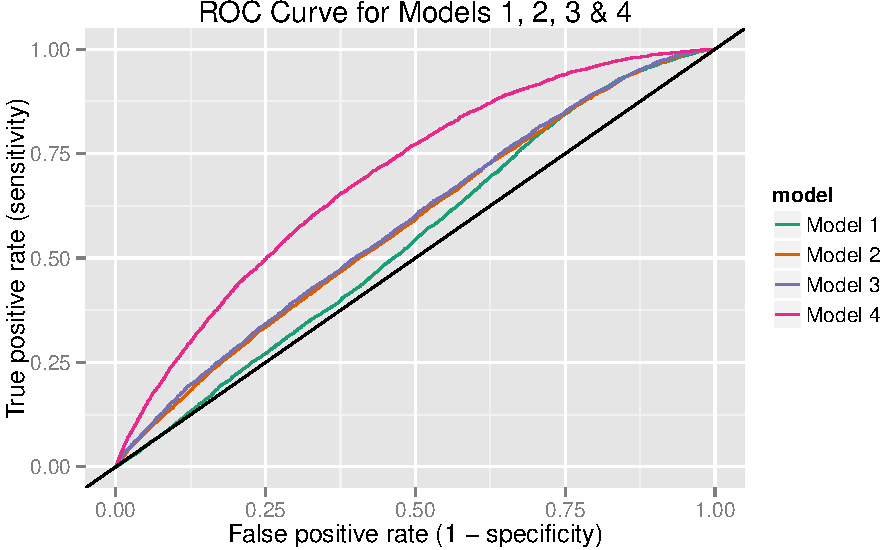
\includegraphics[width=1\columnwidth]{figures/all_roc.pdf} 
	\caption{ROC curve for logistic models} 
	\label{fig:ffdi} 
\end{figure}


Figure \ref{fig:ffdi} is the ROC curve for the four logistic models. The ROC curve for model 1 shows the FFDI is barely better than 'random assignment' (given by 45 degree line) while inclusion of the FFDI inputs and three additional variables improves the ROC curve, clearly the superior model is Model 4. Allowing for variables to have a non-linear effect on the log-odds ratio had improved the prediction accuracy significantly. 

%interesting that ROC plots for 1,2,3 converge at the higher cutoff values while at lower cutoff values appears that extra variables add value?


\subsection{Classification Trees}

As classification trees can be sensitive to the sample used, I constructed several trees on different balanced samples of the data. As each of the trees were structured very similarly I only report two in figure \ref{fig:tree2}. 

% Trees with all variables
\begin{figure}[h]
	\centering 
%	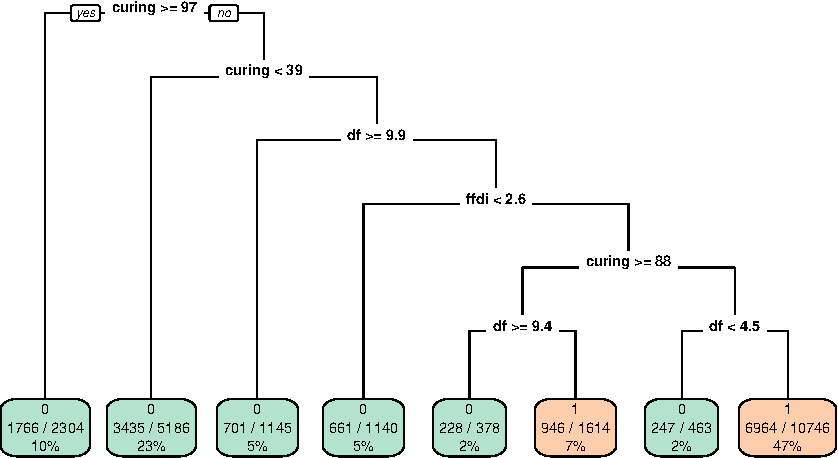
\includegraphics[page=1, width=1\columnwidth]{figures/trees2.pdf} 
%	\includegraphics[page=2, width=1\columnwidth]{figures/trees2.pdf} 
	\caption{Trees with all variables} 
	\label{fig:tree2} 
\end{figure}

For both the reported trees, curing is the first and second split on the tree. When the same variable is used for consecutive splits in a classification tree there are bands of values which the variable takes which are determining the outcome. 

Interpreting the first tree in figure \ref{fig:tree2}, when the grassland curing level is outside the 39 to 97 range the tree predicts there will be no fire. Approximately 33\% of the training data lies in these branches. 

The second and third branch (from the left) contains 5\% of the training data and tells us that when curing lies between 39 and 97 and the drought factor is above 9.9 the tree predicts no fire. If the drought factor is below 9.9 but the FFDI is less than 2.6 the model also predicts no fire. 

The most interesting branch is the far right which contains 47\% of the training data. This branch says if curing is between 39 and 88, the drought factor is between 4.5 and 9.9, the FFDI is above 2.6 then the model predict fire. However this branch only predicts data within the branch with 64\% accuracy. 

The classification tree results reaffirm the results of the spline models in figure \ref{fig:gam_pl} which suggested the effect of curing and drought factor on probability of ignition is not constant at each level of the variable. The bands of values chosen by the tree as having higher probability of ignition vaguely match the shape of the fitted spline functions in Model 4. The tree selecting ranges of variables for which probability of ignition changes suggests there is a  non-linear relationship between some of the explanatory variables and probabiity of ignition. 

%*Interpret trees especially far right branch, majority of data and classfied badly.
%Interesting the bands of curing and df, look kind of like the splines in \ref{fig:gam_pl}

The classification trees consistently place  curing value and drought factor high up in the tree. This makes intuitive sense as both these variables are related to the fuel and the dryness of the available fuel which potentially is more important that the air temperature. Temperature is expected to contribute to probability of ignition but in the longer term. Prolonged high temperatures lead to high curing (drier grass) and higher drought factor level, but according to the classifcation tree, temperature on the particular day is irrelevant. 

%Confusion matrix cutoff=0.5
\begin{table}[ht]
	\centering
	\begin{tabular}{r|rr|rr}
		\hline
		  & Tree 1 &  & Tree 2 & \\ 
		\hline
		& Actual   &  &  &   \\ 
		Predict  & No Fire & Fire & No Fire & Fire\\ 
		\hline
No Fire  & 0.5553 & 0.0017 & 0.5088 & 0.0014 \\ 
Fire  & 0.4394 & 0.0036 & 0.4859 & 0.0038 \\ 
		\hline
	\end{tabular}
	\caption{Confusion Matrices for trees cutoff value 0.5}
	\label{table:tcm2}
\end{table}


% Accuracy for cutoff 0.5
\begin{table}[H]
	\centering
	\begin{tabular}{rrr}
		\hline
		 & Tree 1 & Tree 2 \\ 
		\hline
		Sensitivity  & 0.5582 & 0.5115 \\ 
		Specificity & 0.6832 & 0.7273 \\  
		Balanced Accuracy  & 0.6207 & 0.6194 \\ 
		Accuracy  & 0.5589 & 0.5127 \\ 
		Kappa & 0.0055 & 0.0051 \\ 
		\hline
	\end{tabular}
	\caption{Accuracy for trees cutoff value 0.5}
	\label{table:tacc2}
\end{table}

Tables \ref{table:tcm2} and \ref{table:tacc2} show the confusion matrix and accuracy measures for the classification tree based on the test data. Using a cutoff value of 0.5 the classification trees are comparable to logit models 3 and 4 based on balanced accuracy and incorrectly predicted 'No fires'. 

Based on the ROC plot though the tree is superior to logit model 3 but inferior to the splines model. 


\begin{figure}[h]
	\centering 
%	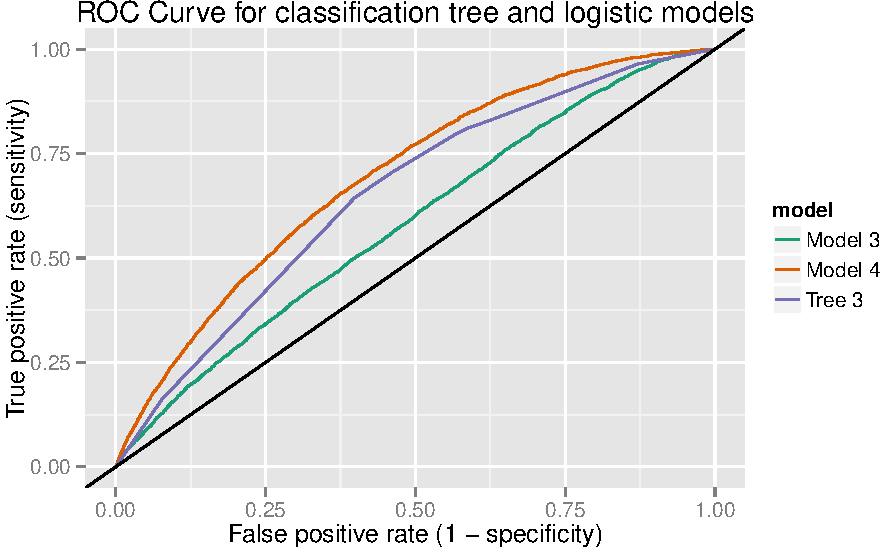
\includegraphics[width=1\columnwidth]{figures/trees_roc.pdf} 
	\caption{ROC curve for Tree Models} 
	\label{fig:troc} 
\end{figure}


\subsection{Random forest}

I produce the random forest using the caret and randomForest packages \citep{caret, rf} in R. The random forest is built using the balanced training set and then assessed on its prediction on the test set. 

Table \ref{table:cmrf} contains the confusion matrix for the forest predictions using a cutoff value of 0.5. Comparing these values to those in table \ref{table:cm2} for model 4 the forest and splines model predict have the same level of accuracy in predicting actual fires. The forest performs slightly better than the splines model at predicting no fires. Accordingly, we observe slightly higher balanced accuracy and kappa. 

%confusion matrix on 0.5 cutoff value
\begin{table}[ht]
	\centering
	\begin{tabular}{rrr}
		\hline
		& Random Forest &  \\ 
		\hline
		& Actual   &   \\ 
		Predict  & No Fire & Fire \\ 
		\hline
		No Fire & 0.6093 & 0.0016 \\ 
		Fire & 0.3856 & 0.0035 \\ 
		\hline
	\end{tabular}
		\caption{Confusion matrix for random forest cutoff value 0.5}
		\label{table:cmrf}
\end{table}

\begin{table}[ht]
	\centering
	\begin{tabular}{rr}
		\hline
		& Random Forest \\ 
		\hline
		Sensitivity & 0.6124 \\ 
		Specificity & 0.6771 \\ 
		Balanced Accuracy & 0.6447 \\ 
		Accuracy & 0.6127 \\ 
		Kappa & 0.0075 \\ 
		\hline
	\end{tabular}
			\caption{Accuracy measure random forest cutoff value 0.5}
			\label{table:accrf}
\end{table}

The variable importance is calculated as mean decrease in accuracy using the out-of-bag observations, described in detail by \cite{archer08}. Figure \ref{fig:vimp} shows the variable importance for the forest. 

Grassland curing is the most important variable in determining fire ignition which is consistent with the output from the individual trees where curing was the first and second split for the majority of the trees. 

FFDI, temperature, vapour pressure, relative humidity and windspeed all have close values of importance. The FFDI is second most important in determining probability of fire ignition which seems counterintuitive given it's poor perfomance in the classification trees and logistic regression. 

Similar variable importance may indicate that on the average across all trees the variables are equally important in determining probability of ignition, however variable importance cannot necessarily be taken simply at face value. \cite{strob07}  and \cite{strob08} show that variable importance measures may be biased by the measurement scale of the variables and show a preference for correlated variables. Alternative calculation of variable importance is outside the scope of this paper but the limitations of the Gini method should be taken into account. 

Table \ref{table:correl} is the cross-correlation matrix for the variables and we observe that many of the variables have relatively high correlation coefficients (with the exception of vapour pressure and windspeed) which may be causing biased variable importance. 


\begin{figure}[h]
	\centering 
%	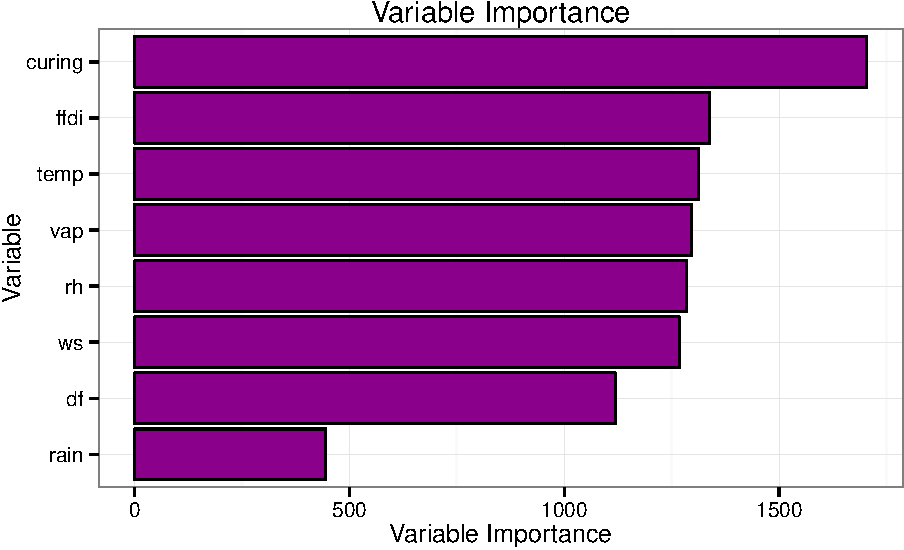
\includegraphics[width=1\columnwidth]{figures/varimp.pdf} 
	\caption{Variable Importance for random forest} 
	\label{fig:vimp} 
\end{figure}

Finally figure \ref{fig:rocrf} shows the ROC curve for the random forest, a single classification tree, the linear logistic model and the splines model. Table \ref{table:AUC} contains the area under the curves (AUC) for the ROC curves shown in \ref{fig:rocrf} . We see the forest and splines model outperform a single tree and linear-logistic model. The closeness of the two models is interesting given random forests are generally expected to be a the best predictors at the expense of interpretability. 

\begin{table}[h]
	\centering
	\begin{tabular}{r|rrrr}
		\hline
		& Model 3 & Model 4 & Tree & Forest \\ 
		\hline
		AUC & 0.58 & 0.69 & 0.65 & 0.70 \\ 
		\hline
	\end{tabular}
	\caption{Areas under ROC curve for logistic model, classification trees \& forest}
	\label{table:AUC}
\end{table}

\begin{figure}[h]
	\centering 
%	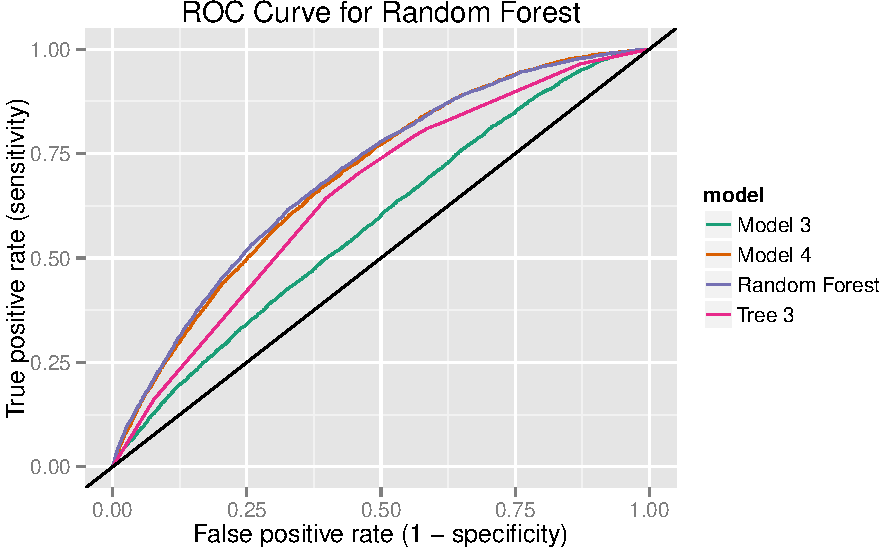
\includegraphics[width=1\columnwidth]{figures/roc_rf.pdf} 
	\caption{Variable Importance for random forest} 
	\label{fig:rocrf} 
\end{figure}

\subsection{Extensions}

This thesis takes a very simplistic view of the dataset, rather than utilising the spatial and time series component, I treat each spatial and time point as independent. Utilising the lagged variables will no doubt improve the model for example we'd expect after a week of hot windy days the probability of ignition would be higher compared to a week of cold days or rain. 

From the Figure \ref{fig:firemap} and the plots of the explanatory variables clearly show a difference in fire behaviour across districts. There is potential for improved accuracy by training different models for the different districts to capture the different conditions in each area. 

Obviously there's more to fire occurence than weather conditions, this study leaves out the essential human component of fire ignition. We see in Figure \ref{fig:firemap} that fire activity corresponds with population density and the major roads in Victoria. The best model in this thesis still only has balanced accuracy of .64 which is a fairly poor model but a more accurate model would indicate overfitting or something else has gone awry.  Weather conditions are important to an extent but we expect them to have greater impact on spread and fire behaviour once ignition has occured rather than ignition itself. 


\section{Conclusion}

This thesis set out to achieve three things:
\begin{enumerate}
\item Evaluate the FFDI as a predictor for bushfire ignition.
\item Identify other variables that will improve ability to predict bushfire ignition.
\item Compare the performance of nonparametric estimation and machine learning techniques to traditional logistic regression.
\end{enumerate}

From the different models in this paper, I conclude that the FFDI alone of a poor predictor of bushfire ignition. 

In the logistic models the first, based only on the FFDI, had very low accuracy when  in predicting the test set and the ROC plot. The FFDI was still statistically significant when the other variables were added but the joint significance of it's inputs even after FFDI was included in the model suggests that the FFDI is not capturing all the information contained in it's inputs. Once n the splines were included the FFDI was no longer statistically significant. 

The single classification trees placed FFDI as very low split which we can interpret as the FFDI not being very helpful in classifying fire occurence. The random forest ranked the importance of the FFDI second highest but given the correlation between the FFDI and its inputs this result is unreliable. 

The logistic model with splines, classification trees and random forest all agreed on the importance of grassland curing in predicting fire ignition. The statistical significance of the spline function of curing in the logistic-spline model, the output of the classification trees consistently placing curing as the highest split and the variable importance ouput from the random forest. While all three additional variables improved accuracy of the models, grassland curing was clearly superior. 

This paper has clearly demonstrated the benefit of combining variables differently to the linear construction typically seen in standard logistic models. Both regression splines and algorithmic techniques in improving predictive models. Ranking by accuracy on the test set, the random forest and spline models performed the best followed by a single classification tree. All three models were superior to the standard logistic regression. 

The interesting result is the similarity in perfomance of the splines model and the random forest. Using splines to allow a non-linear relationship between the log-odds ratio and the variables while random forests typically capture interactions between variables. Both these mathods led to a large improvement in the predictive perfomance.

This analysis provides a solid baseline for further study. Having shown alternate statistical techniques which capture more of the complexity and interactions in this problem and developed a model which although difficult to interpret, performs strongly in the test data. 

\section*{Acknowledgment}
\textit{No one who achieves success does so without acknowledging the help of others. The wise and confident acknowledge this help with gratitude. -Alfred North Whitehead
	}
	
I am indebted to my indefatigable supervisors Rob and Di, thank you for your endless patience. 

To those who I adopted as my pseudo-supervisors Souhaib Ben-Taieb, Klaus Ackerman, Simon Angus, your help and advice was invaluable.

To my biggest supporters Earo Wang \& Christien Blencowe without your encouragement, your help and Earo's endless of chocolate this year would have been impossible.

Special thanks to Sarah Harris (Earth \& Atmosphereic Science, Monash), Hamish Clarke (UNSW), Stuart Matthews (Rural Fire Service, NSW), Musa Kilinc \& Danielle Wright (Country Fire Authority), who all contributed with data and helpful advice.

To my long suffering honours cohort, I apologise for the tears and for boring you with my data struggles, you have been the the best team to be a part of. 

% Appendices start here
\bibliographystyle{agsm}

\bibliography{references}


\end{document}
